%\info{Andrew, Simone}

\subsection{Analytics}

\info{IAN}

Should try to get to the point where we can say something about where the sensitivity in the distribution comes from (e.g. slope in log scale is proportional to $C_F\times \alpha_s$).  At the very least, it would be good to write down the LL (or even NLL) functional form for the angularities that we used (it is in the code we got from Ian (LL) and Gregory (NLL)).  Could also punt this to Sec.~\ref{sec:templates} where we will show the templates (could then just give a ref).

\begin{comment}
The Soft Drop grooming procedure~\cite{Larkoski:2014wba} takes a jet
with momentum $p_t$ and radius $R$. It re-clusters its constituents
using the Cambridge/Aachen (C/A) algorithm \cite{Dokshitzer:1997in,
  Wobisch:1998wt} and iteratively performs the following steps:
\begin{enumerate}
 \item it de-clusters the jet into 2 subjets $j \to j_1 + j_2$;
 \item it checks the condition 
\begin{equation}\label{eq:sd-condition}
\frac{\min (p_{t1} , p_{t2})}{p_{t1}+p_{t2}} > \zcut \left(
  \frac{\theta_{12}}{R}\right)^\beta\,;
\end{equation}
\item if the jet passes the condition, the recursion stops; if not the
  softer subjet is removed and the algorithms goes back to step 1 with
  the hardest of the two subjets. 
 \end{enumerate}
In the case $\beta=0$ Soft Drop essentially reduces to mMDT~\cite{Dasgupta:2013ihk},
 albeit without any actual mass-drop condition. Moreover, while the
 original MDT~\cite{Butterworth:2008iy} algorithm imposed a cut on the ratio of angular distances
 to masses, a so-called $\ycut$, the mMDT variant instead cuts on
 momentum fractions~\cite{Dasgupta:2013ihk} (see
 e.g. \cite{Dasgupta:2013ihk,Dasgupta:2016ktv} for a comparison
 between $\ycut$ and $\zcut$).
 \end{comment}

Notes (order not meaningful): Plot of the two calculations for softdrop mass?  Show plots of the ATLAS and CMS measurements?  Actually, I'm not sure we can show CMS since it is only preliminary.  Say something about mass versus $k_t$?

\subsection{Parton Shower Monte Carlo Studies}

\info{BEN}

From the point of view of fitting for $\alpha_s$, a good observable is one whose probability distribution changes significantly with variations in $\alpha_s$.  However, many observables that significantly change with $\alpha_s$ are also very sensitive to non-perturbative effects, such as the multiplicity inside jets.  In this section, many angularities are studied to quantify the tradeoff between the sensitivity to $\alpha_s$ and the robustness to non-perturbative effects.  Given two probability distributions $f$ and $g$, define the separation power $\Delta(f,g)$~\cite{Harrison:1998yr} as

\begin{align}
\label{eq:seppower}
\Delta(f,g)=\frac{1}{2}\int d\lambda \frac{(f(\lambda)-g(\lambda)^2}{f(\lambda)+g(\lambda)}.
\end{align}

\noindent As defined by Eq.~\ref{eq:seppower}, the separation power is a number in $[0,1]$ where $\Delta=1$ if and only if $f=g$ a.e.  If $f$ is the nominal probability distribution of some observable and $g$ the distribution of the same observable with a different value of $\alpha_s$, we would like $\Delta(f,g)$ close to 1.  In contrast, if $g$ is the same as $f$ with some variation in the non-perturbative effects, then we would like $\Delta(f,g)$ to be close to $0$.  The plane used to study the tradeoff between sensitivity and robustness is shown in Fig.~\ref{fig:robustnessschematic}.  Not all information about $\alpha_s$ sensitivity is captured by a single point in Fig.~\ref{fig:robustnessschematic} because sensitivity to non-perturbative effects could be in regions of low $\alpha_s$ sensitivity and vice versa.  Therefore, it is also useful to study the integrand of Eq.~\ref{eq:seppower} as a function of the angularity $\lambda$.

\begin{figure}[h!]
\begin{center}
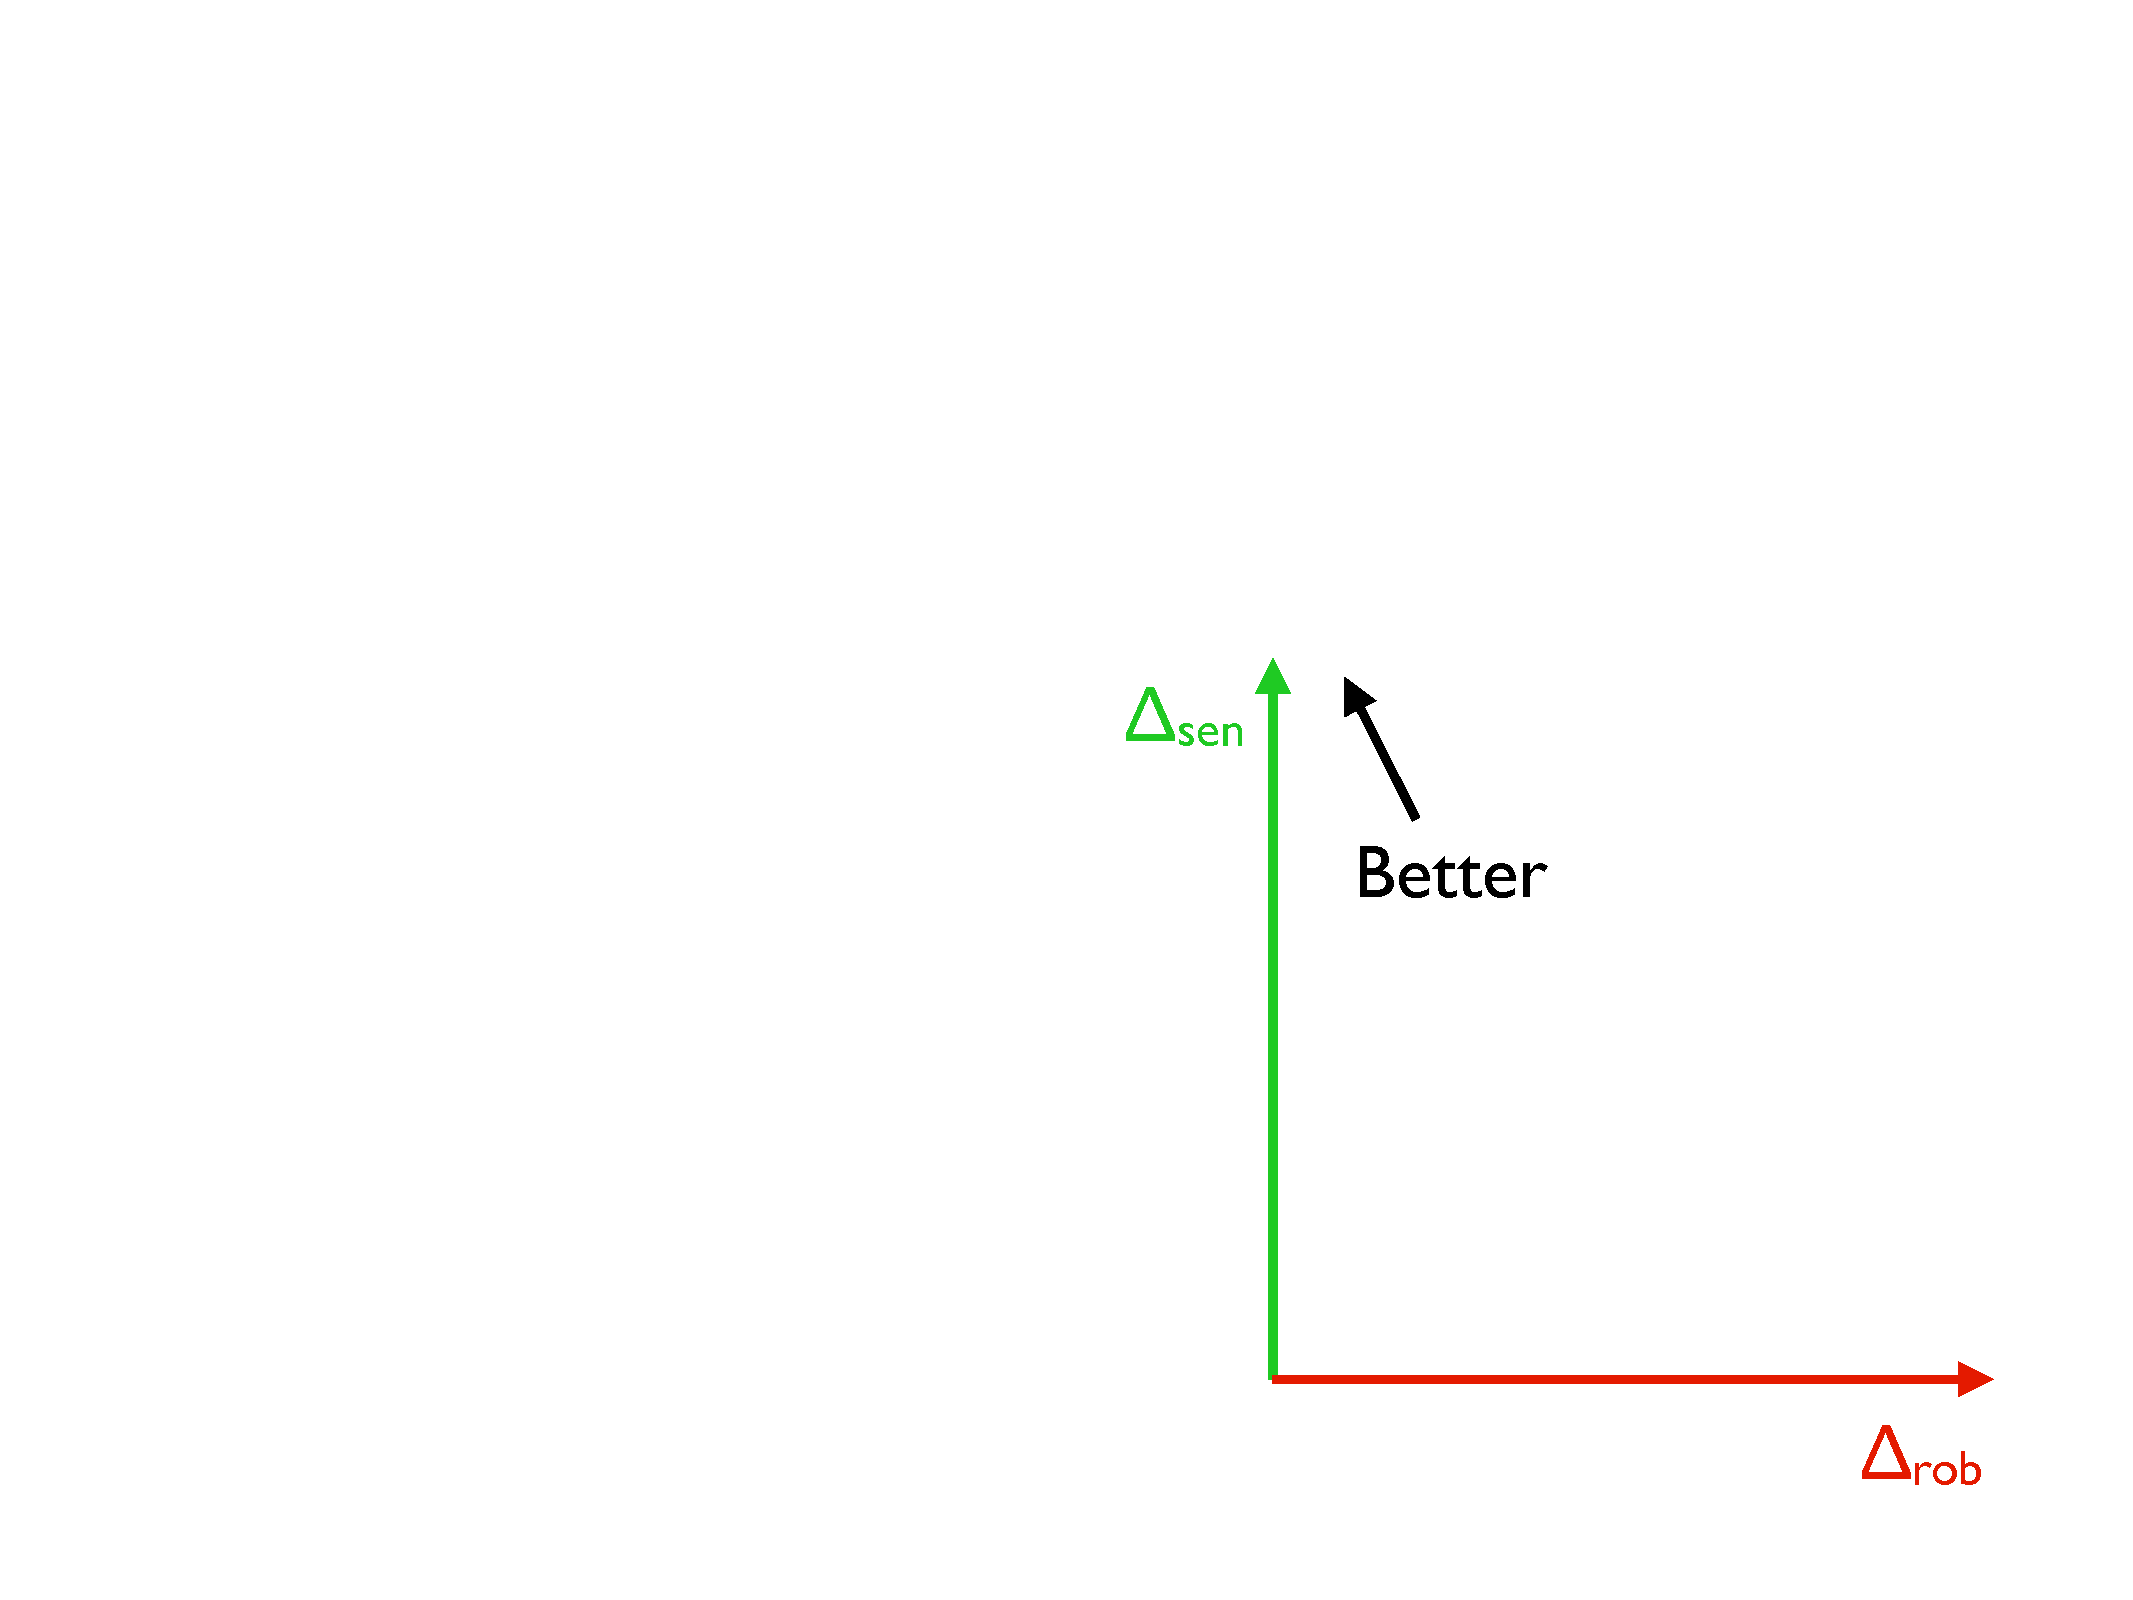
\includegraphics[width = 0.4\columnwidth]{figures/robustnessschematic.pdf}
\end{center}
\caption{A schematic diagram to illustrate the sensitivity-robustness plane defined by the separation power defined in Eq.~\ref{eq:seppower}.}
\label{fig:robustnessschematic}
\end{figure}

The sensitivity-robustness tradeoff is studied using (formally) leading logarithm PS MC programs Herwig 7.1~\cite{Bellm:2015jjp,Reichelt:2017hts} with the default tune and Pythia 8.223~\cite{Sjostrand:2006za,Sjostrand:2014zea} with the tune 4C.  Results are presented for separately for quark and gluon jets, simulated with $Z+q$ and $Z+g$.  A variety of angularities $e_\alpha=\sum_iz_i\theta_i^\alpha$ were studied, with $\alpha\in\{0.5,1.0, 2.0\}$ corresponding to the Les Houches Angularity~\cite{Gras:2017jty}, width, and mass, respectively.  Additionally, various grooming parameters are studied by varying $\beta\in\{0,1,2\}$ and $z_\text{cut}\in 0.05,0.1,0.2\}$.  

Figures~\ref{fig:sensitivity} and~\ref{fig:robustness} show BLAH.

\begin{figure}[h!]
\begin{center}
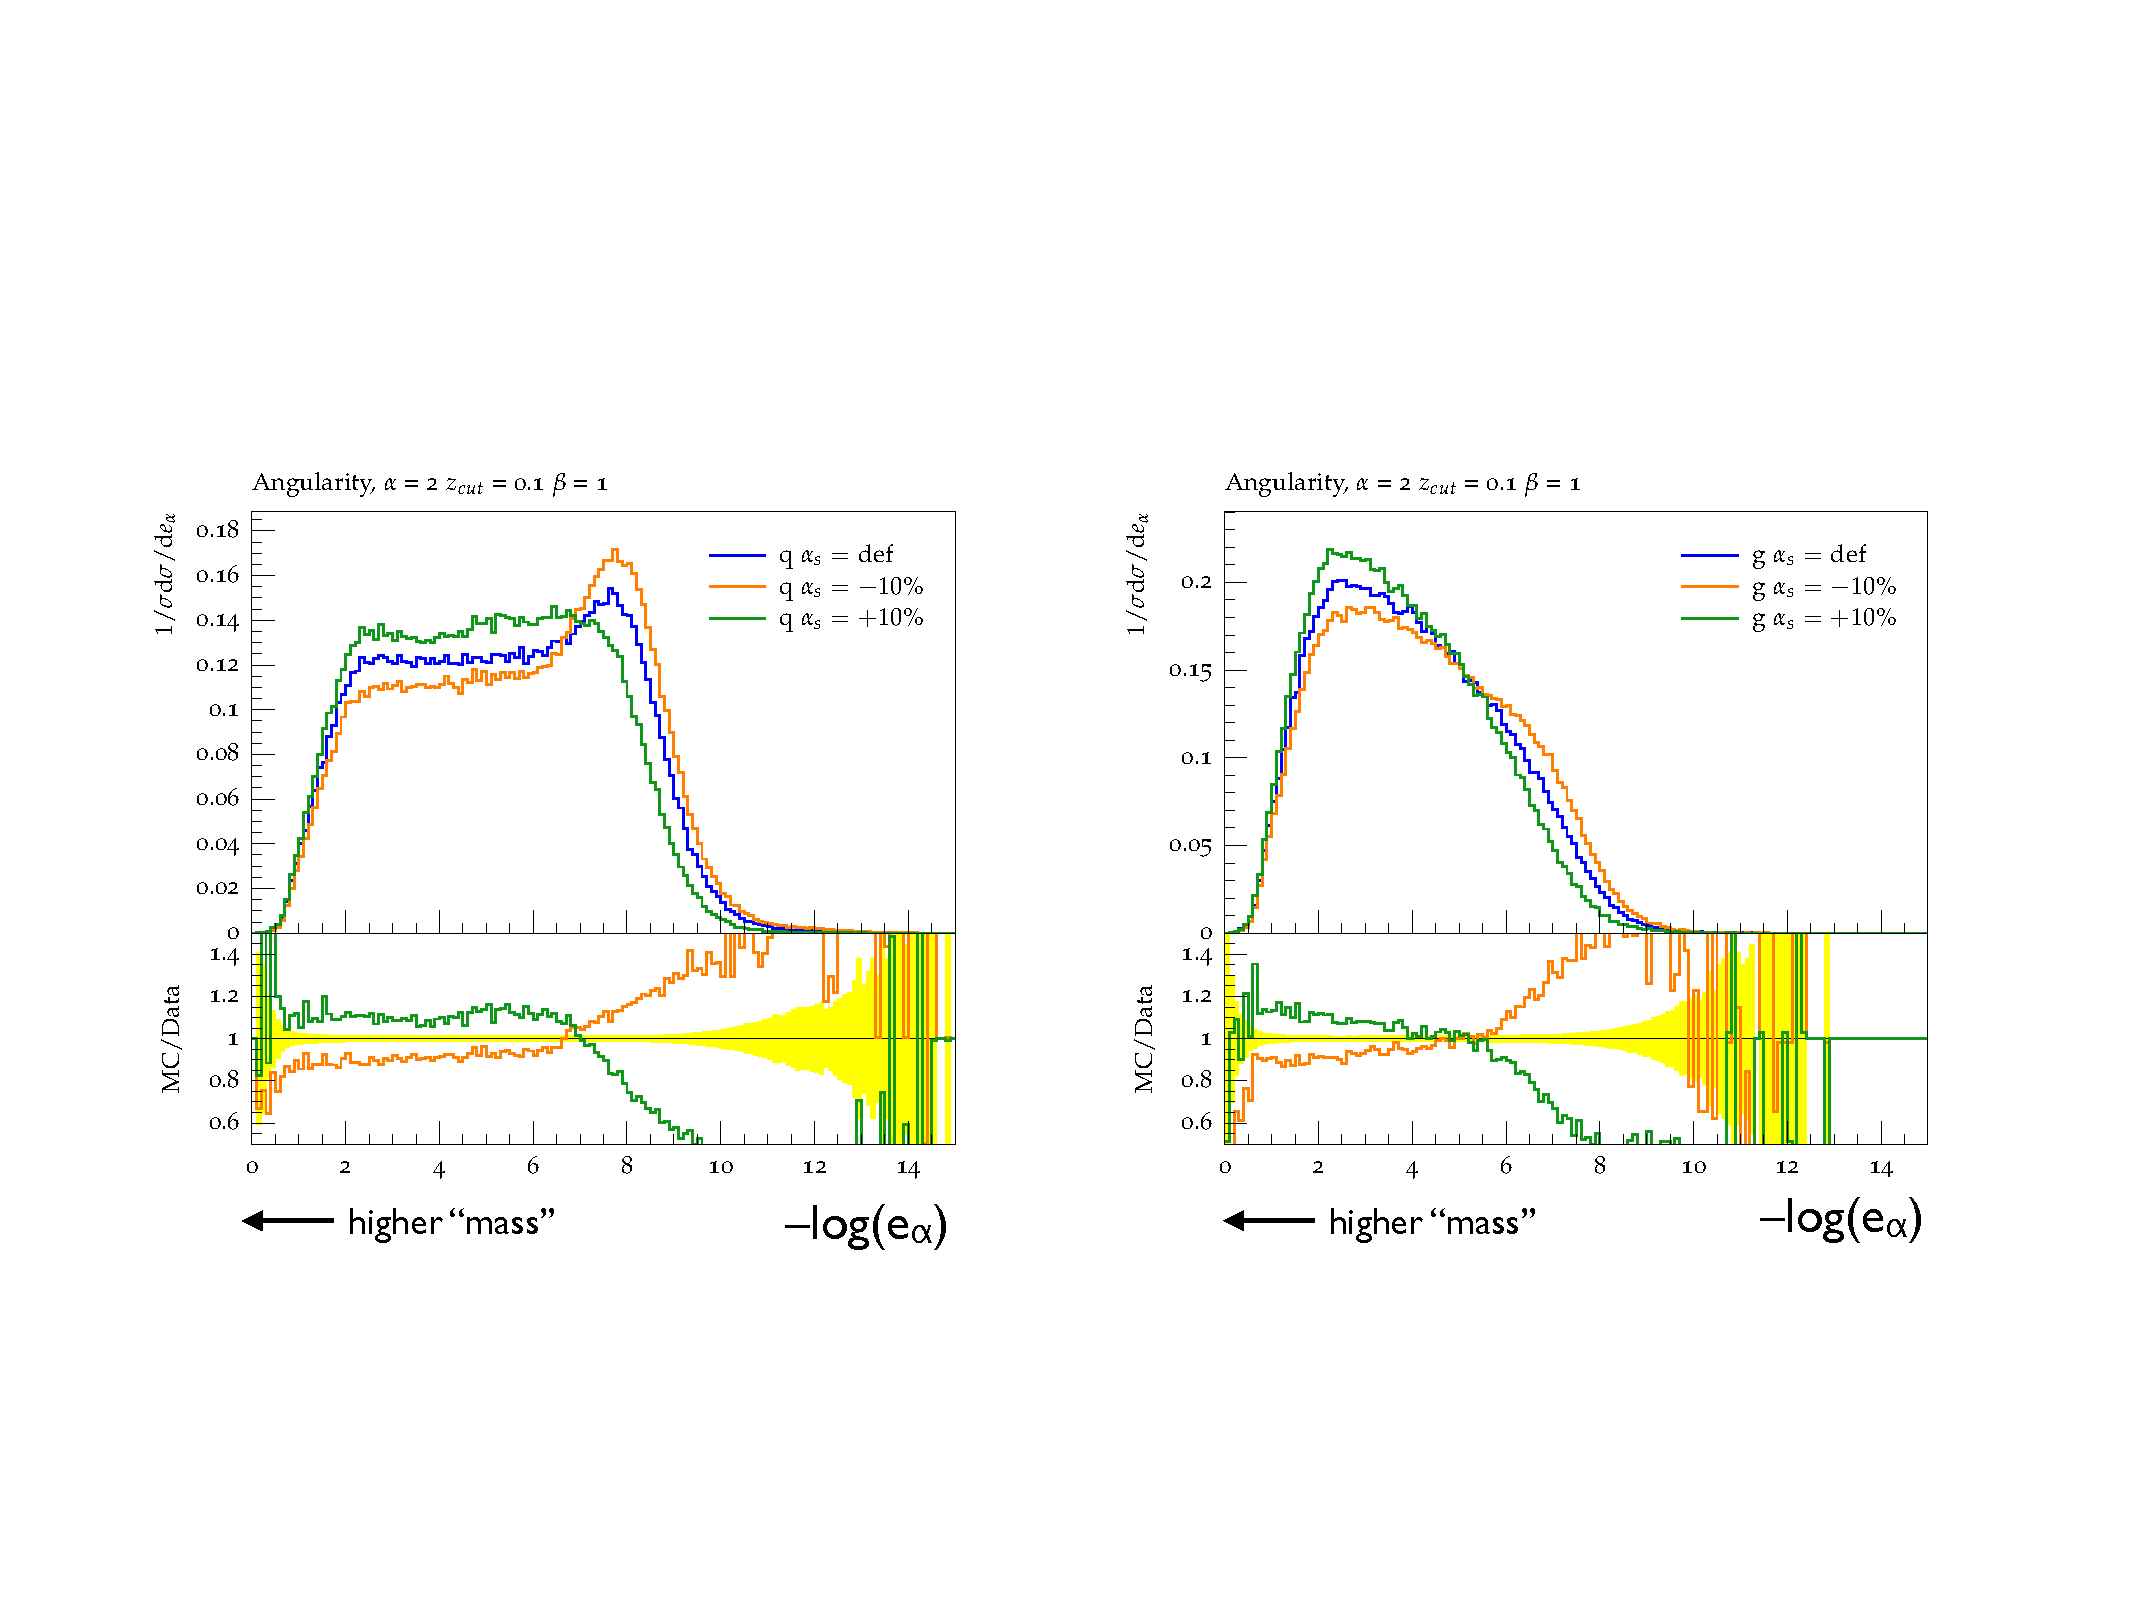
\includegraphics[width = 0.99\columnwidth]{figures/sensitivity.pdf}
\end{center}
\caption{The distribution of the normalized squared jet mass ($e_2$) for quark jets (left) and gluon jets (right).  Higher values of the mass are on the left.  The blue line uses $\alpha_s=0.118$ while the green and orange lines have the value of $\alpha_s$ varied by $10\%$.  The lower panels show the ratio with respect to the $\alpha_s=0.118$ curve.}
\label{fig:sensitivity}
\end{figure}

\begin{figure}[h!]
\begin{center}
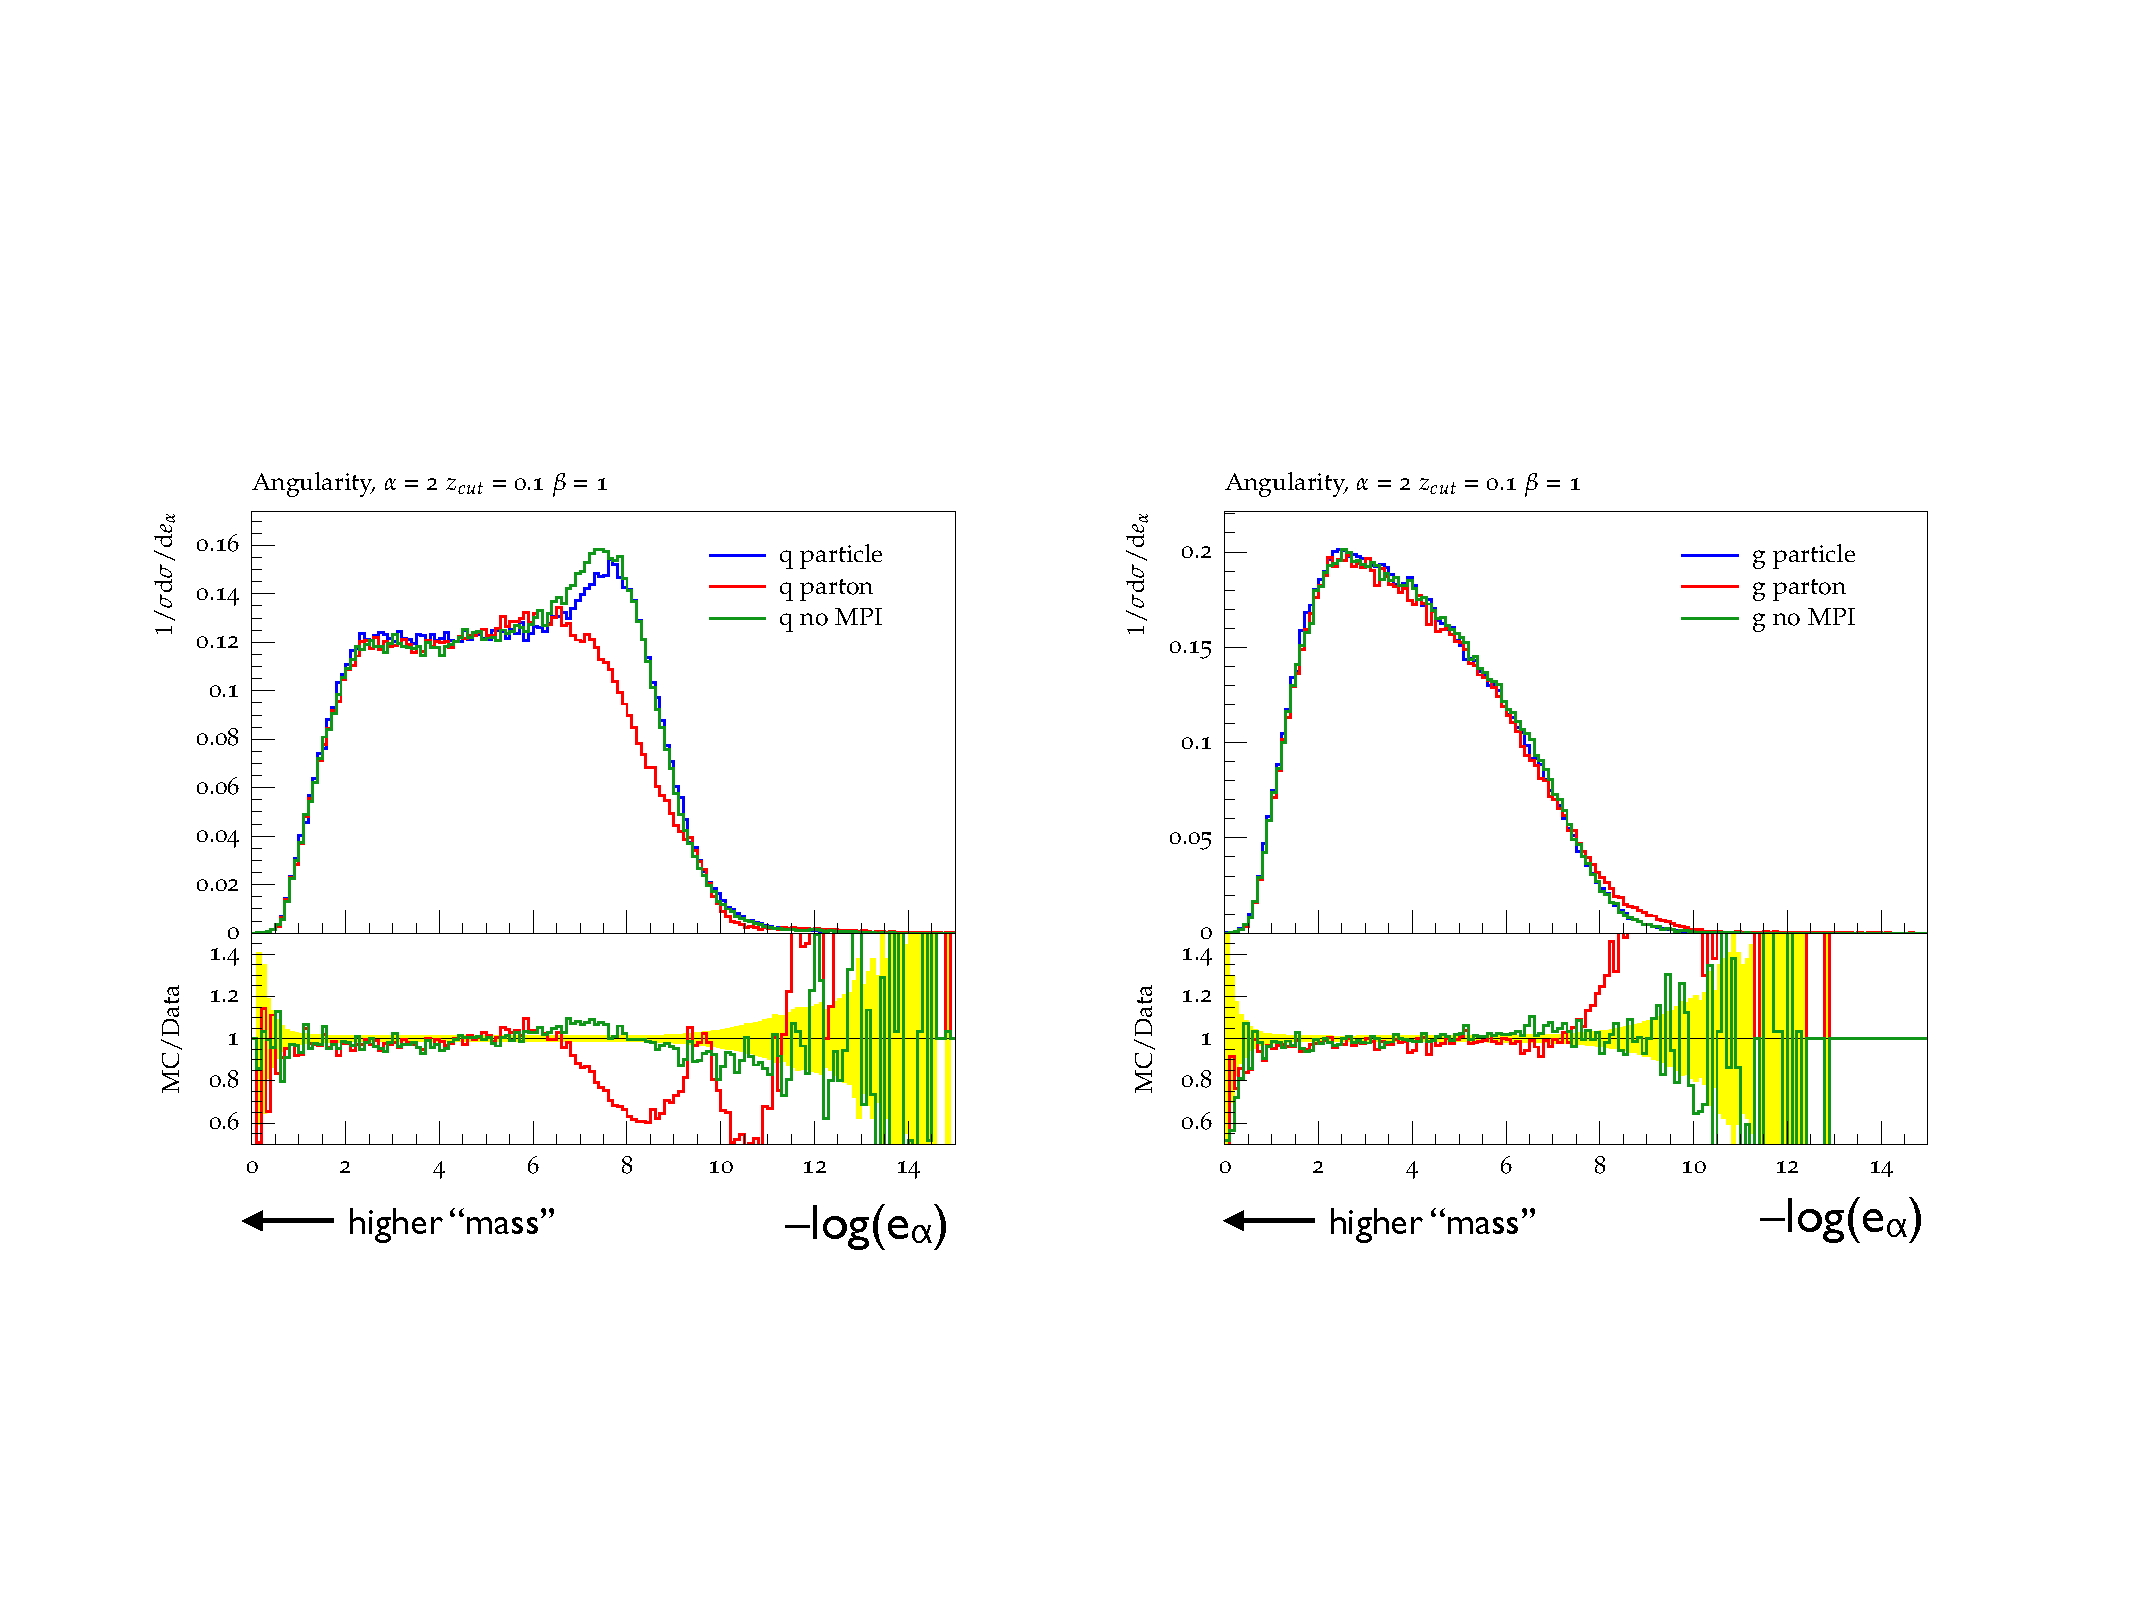
\includegraphics[width = 0.99\columnwidth]{figures/robustness.pdf}
\end{center}
\caption{The distribution of the normalized squared jet mass ($e_2$) for quark jets (left) and gluon jets (right).  Higher values of the mass are on the left.  The blue line shows the default particle-level simulation that includes the standard cluster hadronization model.  The red curve has hadronization turned off and the green curve has hadronization, but with the Herwig model for multiple parton interactions (MPI) turned off.}
\label{fig:robustness}
\end{figure}

\begin{figure}[h!]
\begin{center}
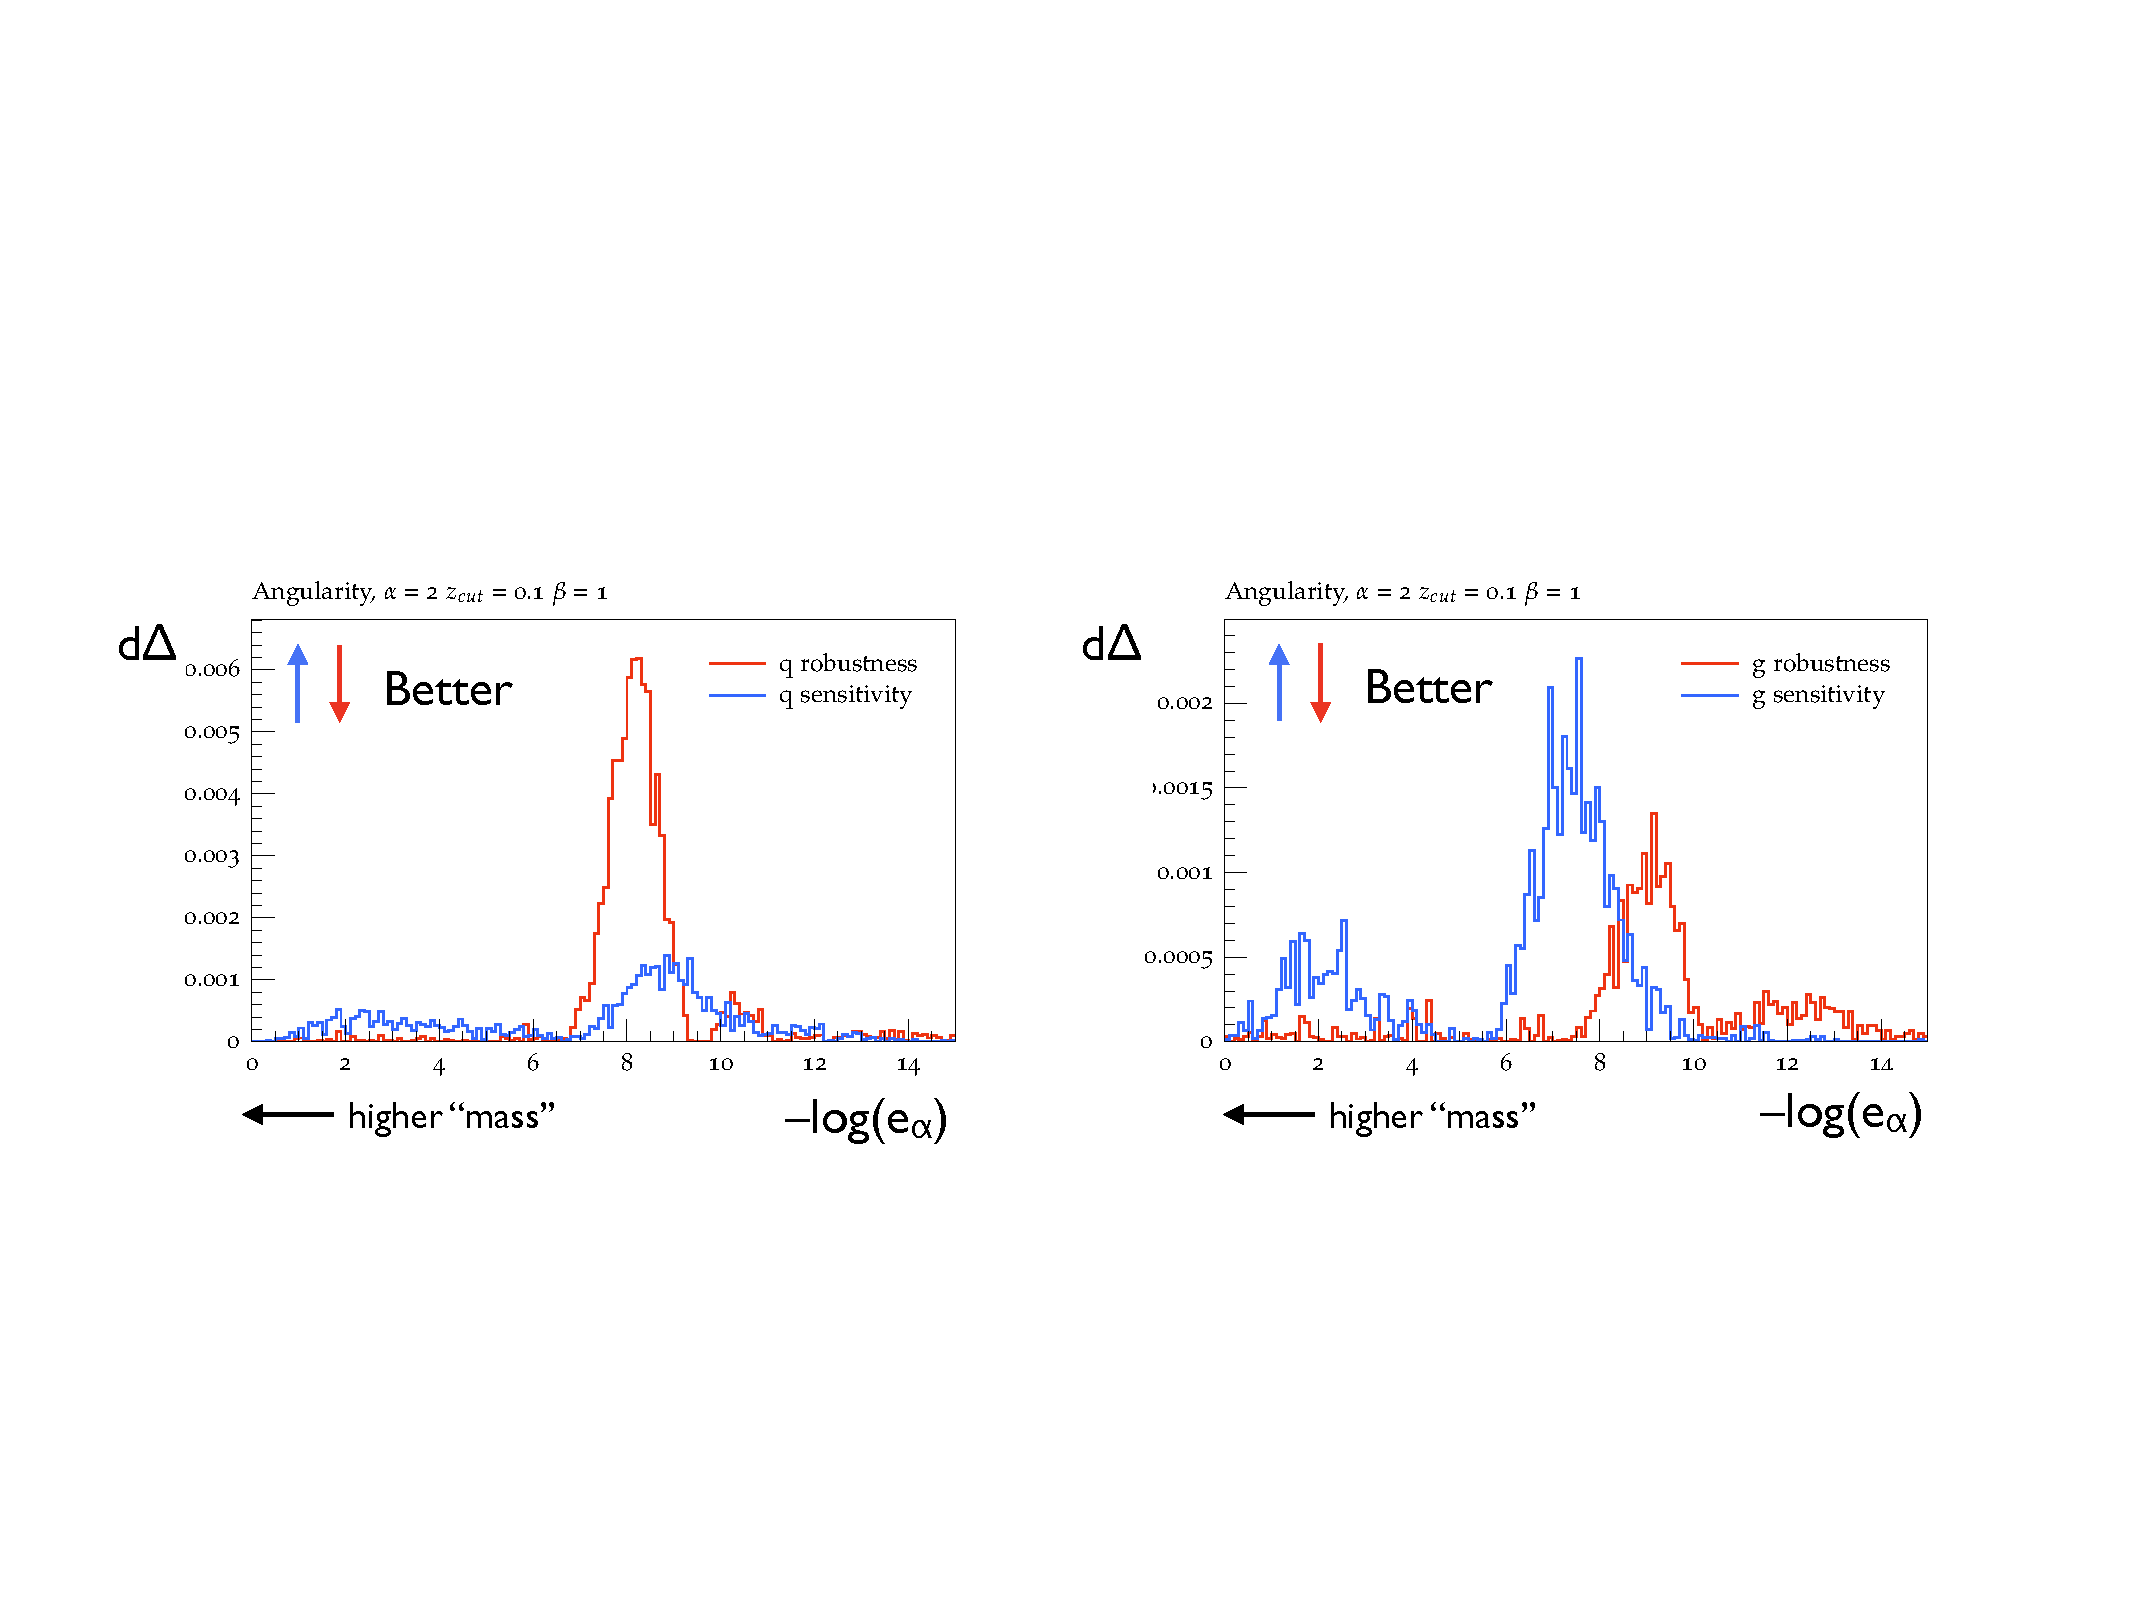
\includegraphics[width = 0.99\columnwidth]{figures/differentialseparation.pdf}
\end{center}
\caption{The integrand of Eq.~\ref{eq:seppower} for the normalized squared jet mass ($e_2$) for quark jets (left) and gluon jets (right).  Higher values of the mass are on the left.  In $f$ from Eq.~\ref{eq:seppower} is the same for red and blue, but for blue (robustness), $\alpha_s$ is varied by 10\% and for red (robustness), hadronization is turned off.}
\label{fig:differentialseparation}
\end{figure}

\begin{figure}[h!]
\begin{center}
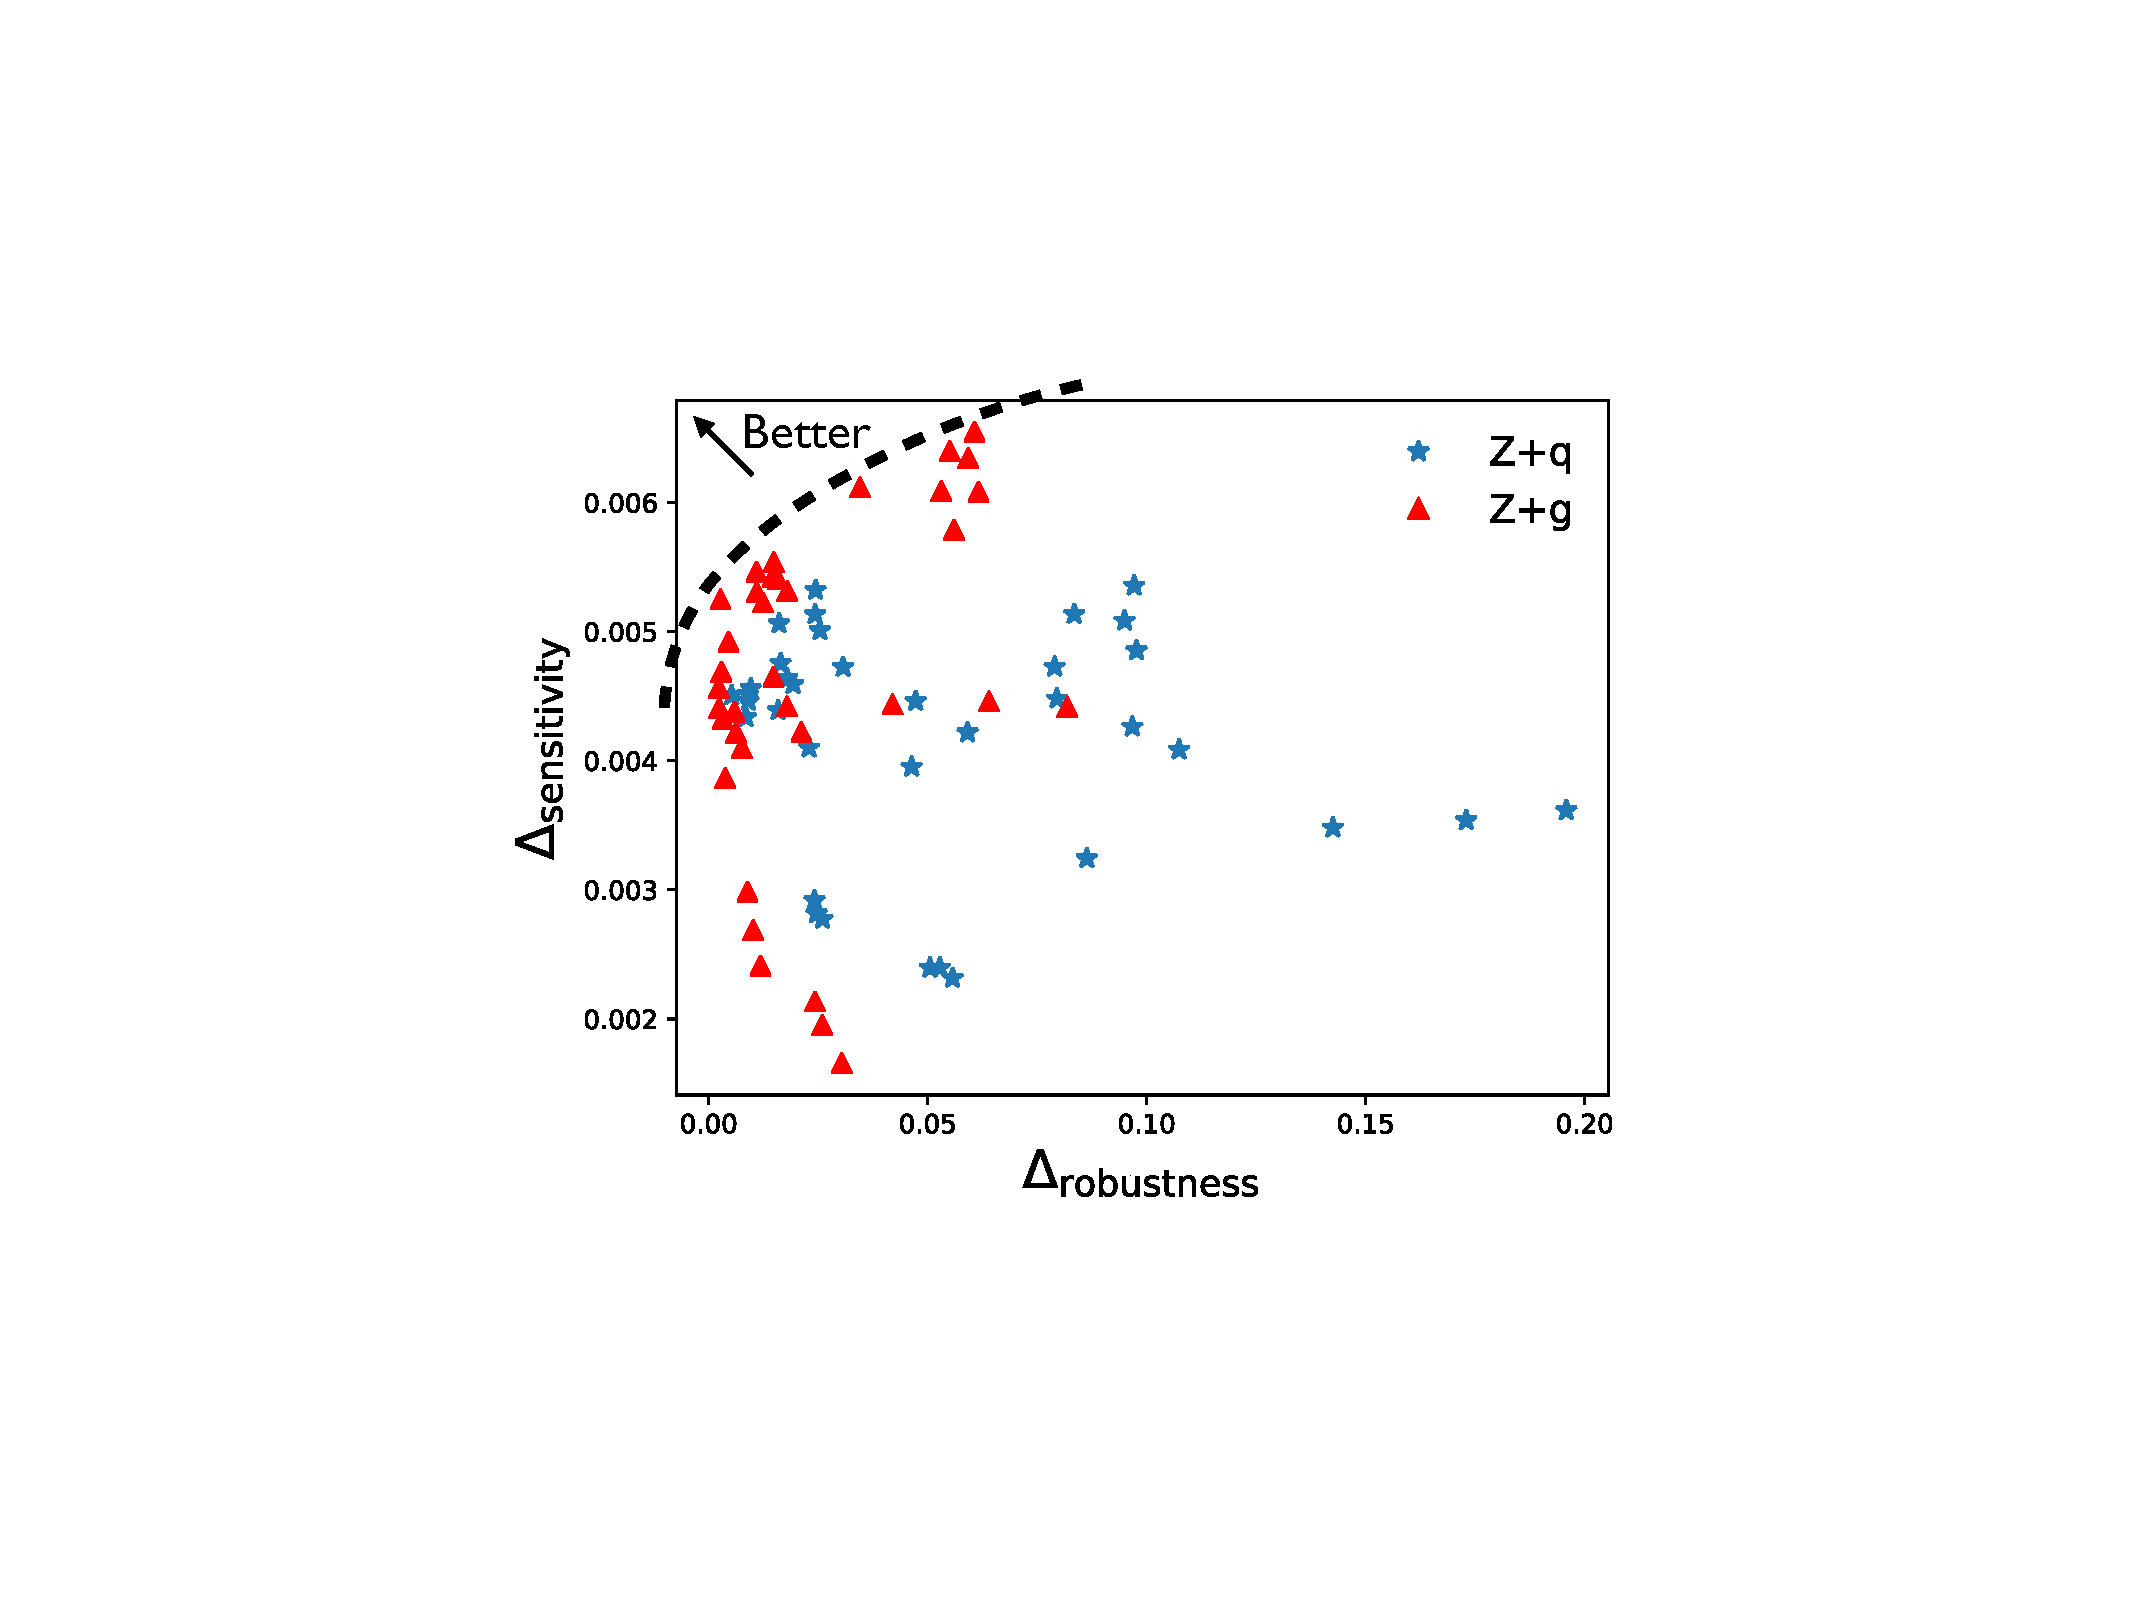
\includegraphics[width = 0.6\columnwidth]{figures/robseptradeoff.pdf}
\end{center}
\caption{The tradeoff between sensitivity and robustness for the 36 angularities studied in this section.  Stars represent quark jets and triangles represent gluon jets.}
\label{fig:robseptradeoff}
\end{figure}
